\documentclass[border=8pt]{standalone}
\usepackage{tikz}
\usetikzlibrary{arrows.meta, positioning, calc, backgrounds}

% Colours
\definecolor{meat}{RGB}{205,75,75}
\definecolor{veg}{RGB}{75,165,75}
\definecolor{debit}{RGB}{190,50,50}
\definecolor{panelbg}{RGB}{248,248,248}
\definecolor{severed}{RGB}{160,160,160}

\begin{document}
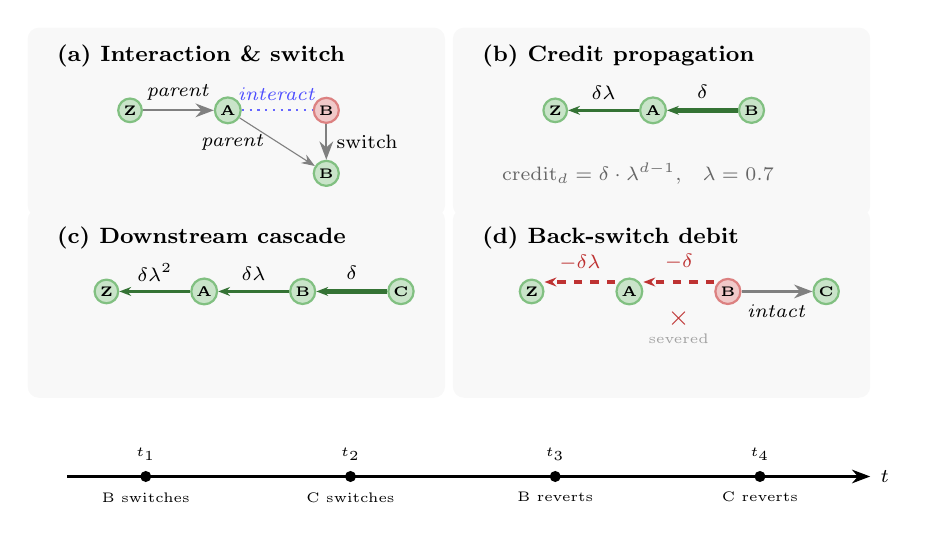
\begin{tikzpicture}[
    node distance=0.7cm and 0.9cm,
    agent/.style={circle, draw, thick, minimum size=0.27cm, inner sep=1pt, font=\tiny\bfseries},
    meatnode/.style={agent, fill=meat!30, draw=meat!70},
    vegnode/.style={agent, fill=veg!30, draw=veg!70},
    credit/.style={-{Stealth[length=1.5mm]}, veg!70!black, thick},
    debitarrow/.style={-{Stealth[length=1.5mm]}, debit, thick, dashed},
    lbl/.style={font=\scriptsize, text=black},
    paneltitle/.style={font=\footnotesize\bfseries, anchor=north west},
]

\def\panelw{4.8}
\def\panelh{1.9}
\def\gaph{0.4}
\def\gapw{0.6}

% ===== PANEL (a): Switch Event =====
\begin{scope}[shift={(0,0)}]
  \begin{scope}[on background layer]
    \fill[panelbg, rounded corners=4pt] (-0.5, -0.5) rectangle (\panelw, \panelh);
  \end{scope}
  \node[paneltitle] at (-0.25, \panelh-0.1) {(a) Interaction \& switch};

  % Before: Z--A  A...B(meat)
  \node[vegnode] (Z1) at (0.8, 0.85) {Z};
  \node[vegnode, right=of Z1] (A1) {A};
  \node[meatnode, right=of A1] (B1) {B};

  \draw[-{Stealth}, gray, thick] (Z1) -- (A1) node[midway, above, lbl] {\textit{parent}};
  \draw[dotted, thick, blue!60] (A1) -- (B1)
    node[midway, above, lbl, text=blue!70] {\textit{interact}};

  % After: B switches to veg, shown below with arrow
  \node[vegnode] (B1n) at ($(B1)+(0,-0.8)$) {B};
  \draw[-{Stealth}, thick, black!50] (B1) -- (B1n)
    node[midway, right, lbl] {switch};

  % New parent edge
  \draw[-{Stealth}, gray] (A1) -- (B1n) node[midway, left, lbl, xshift=-1pt] {\textit{parent}};


\end{scope}

% ===== PANEL (b): Credit Propagation =====
\begin{scope}[shift={(\panelw+\gapw, 0)}]
  \begin{scope}[on background layer]
    \fill[panelbg, rounded corners=4pt] (-0.5, -0.5) rectangle (\panelw, \panelh);
  \end{scope}
  \node[paneltitle] at (-0.25, \panelh-0.1) {(b) Credit propagation};

  \node[vegnode] (Z2) at (0.8, 0.85) {Z};
  \node[vegnode, right=of Z2] (A2) {A};
  \node[vegnode, right=of A2] (B2) {B};

  % Credit arrows — thickness encodes decay
  \draw[credit, line width=1.8pt] (B2) -- (A2)
    node[midway, above, lbl] {$\delta$};
  \draw[credit, line width=1.2pt] (A2) -- (Z2)
    node[midway, above, lbl] {$\delta\lambda$};

  % Decay formula
  \node[font=\scriptsize, anchor=west, text=black!60] at (0.0, 0.05)
    {$\mathrm{credit}_d = \delta \cdot \lambda^{d-1}$, \; $\lambda = 0.7$};
\end{scope}

% ===== PANEL (c): Downstream Cascade =====
\begin{scope}[shift={(0, -\panelh-\gaph)}]
  \begin{scope}[on background layer]
    \fill[panelbg, rounded corners=4pt] (-0.5, -0.5) rectangle (\panelw, \panelh);
  \end{scope}
  \node[paneltitle] at (-0.25, \panelh-0.1) {(c) Downstream cascade};

  \node[vegnode] (Z3) at (0.5, 0.85) {Z};
  \node[vegnode, right=0.9cm of Z3] (A3) {A};
  \node[vegnode, right=0.9cm of A3] (B3) {B};
  \node[vegnode, right=0.9cm of B3] (C3) {C};

  % Credit arrows — C's switch propagates up full chain
  \draw[credit, line width=1.8pt] (C3) -- (B3)
    node[midway, above, lbl] {$\delta$};
  \draw[credit, line width=1.2pt] (B3) -- (A3)
    node[midway, above, lbl] {$\delta\lambda$};
  \draw[credit, line width=0.8pt] (A3) -- (Z3)
    node[midway, above, lbl] {$\delta\lambda^2$};

\end{scope}

% ===== PANEL (d): Back-Switch Debit =====
\begin{scope}[shift={(\panelw+\gapw, -\panelh-\gaph)}]
  \begin{scope}[on background layer]
    \fill[panelbg, rounded corners=4pt] (-0.5, -0.5) rectangle (\panelw, \panelh);
  \end{scope}
  \node[paneltitle] at (-0.25, \panelh-0.1) {(d) Back-switch debit};

  \node[vegnode] (Z4) at (0.5, 0.85) {Z};
  \node[vegnode, right=0.9cm of Z4] (A4) {A};
  \node[meatnode, right=0.9cm of A4] (B4) {B};
  \node[vegnode, right=0.9cm of B4] (C4) {C};

  % Debit arrows — shifted above centre line
  \draw[debitarrow, line width=1.8pt] ($(B4.west)+(0,0.12)$) -- ($(A4.east)+(0,0.12)$)
    node[midway, above, lbl, text=debit] {$-\delta$};
  \draw[debitarrow, line width=1.2pt] ($(A4.west)+(0,0.12)$) -- ($(Z4.east)+(0,0.12)$)
    node[midway, above, lbl, text=debit] {$-\delta\lambda$};

  % Severed marker below centre line
  \node[font=\normalsize, text=debit] at ($(A4)!0.5!(B4)+(0,-0.35)$) {$\times$};
  \node[font=\tiny, text=severed] at ($(A4)!0.5!(B4)+(0,-0.6)$) {severed};

  % C still linked to B
  \draw[-{Stealth}, gray, thick] (B4) -- (C4)
    node[midway, below, lbl, yshift=-1pt] {\textit{intact}};

\end{scope}

% ===== Timeline strip =====
\begin{scope}[shift={(0, -2*\panelh - 2*\gaph + 0.8)}]
  \draw[thick, -{Stealth}] (0,0) -- (10.2, 0) node[right, font=\scriptsize] {$t$};
  \foreach \x/\lab/\desc in {
    1.0/$t_1$/B switches,
    3.6/$t_2$/C switches,
    6.2/$t_3$/B reverts,
    8.8/$t_4$/C reverts%
  }{
    \fill (\x, 0) circle (2pt);
    \node[above, font=\tiny\bfseries] at (\x, 0.08) {\lab};
    \node[below, font=\tiny] at (\x, -0.08) {\desc};
  }
\end{scope}

\end{tikzpicture}
\end{document}
